\documentclass[11pt]{article}
\usepackage[a4paper,margin=1in]{geometry}
\usepackage{fontspec}
\setmainfont{TeX Gyre Termes}
\usepackage{booktabs}
\usepackage{tabularx}
\usepackage{longtable}
\usepackage{array}
\usepackage{ragged2e}
\usepackage{amsmath}
\usepackage{hyperref}
\usepackage{xcolor}
\usepackage{tikz}
\usetikzlibrary{positioning,shapes.geometric}
\usepackage{caption}
\usepackage{float}

\hypersetup{colorlinks=true,linkcolor=blue,citecolor=blue,urlcolor=blue}
\newcolumntype{Y}{>{\RaggedRight\arraybackslash}X}

\title{Protocol-Aware Observability for AI Chat Streaming:\\
A Systematic Review of Tracing and Metrics for\\
Server-Sent Events and WebSocket}
\author{Undergraduate Research Draft}
\date{June 2026}

\begin{document}
\maketitle

\begin{abstract}
AI chatbot and retrieval-augmented generation (RAG) systems stream responses token-by-token so users see partial output early. Developers often default to WebSocket, yet for server-to-client text generation, Server-Sent Events (SSE) is frequently sufficient and simpler. Observability, however, is harder for both: REST tracing relies on per-request HTTP headers, but once an SSE or WebSocket connection is established, individual events or messages no longer carry HTTP headers, so request-level instrumentation cannot see token-level behaviour. This paper reports a systematic, PRISMA-guided review of how SSE and WebSocket are compared and observed, focusing on the metrics used for streaming AI workloads. We find that (i) token-level metrics --- time to first token (TTFT), inter-token latency (ITL), and output throughput --- are well defined in the LLM-serving literature; (ii) transport-level differences between SSE and WebSocket are minor for one-way token streaming; and (iii) no existing work provides a unified, backend-independent, agent-free instrumentation model that captures token-level observability across both protocols. We synthesise these gaps into a five-layer protocol-aware observability framework and a prototype scope for a Java/Spring~Boot library. This is a preliminary review: experimental measurement is reported as a planned prototype rather than completed results.
\end{abstract}

\textit{Keywords:} Server-Sent Events, WebSocket, observability, distributed tracing, OpenTelemetry, LLM streaming, time to first token, PRISMA.

%==============================================================
\section{Introduction}

\subsection{Rationale}
Modern chatbot and RAG applications stream responses progressively so that users can read partial output before generation completes. Many developers assume such systems must use WebSocket because it supports bidirectional real-time communication. However, for AI text streaming the dominant pattern is one-way server-to-client delivery of generated tokens, for which SSE can be sufficient and operationally simpler. Both OpenAI and Anthropic expose their streaming APIs over SSE \cite{buildmvpfast2026,procedure2026}.

From an observability perspective, REST APIs are straightforward to trace because every request carries headers such as \texttt{traceparent}. SSE and WebSocket, by contrast, are long-lived connections: headers are present only at connection setup, and subsequent events or messages do not automatically carry HTTP headers \cite{w3ctrace,oneuptimews2026}. Tracing streaming systems therefore requires additional connection- and message-level context propagation. This is a practical gap: existing tools trace REST and database calls well, but tracing the lifecycle of SSE and WebSocket streams --- connection open, per-token delivery, disconnects, cross-service propagation --- is less direct.

\subsection{Objectives and Research Questions}
This review studies how SSE and WebSocket are compared and observed for AI streaming, and what gaps remain. It addresses:
\begin{enumerate}
\item \textbf{RQ1}: What metrics are commonly used to compare SSE and WebSocket?
\item \textbf{RQ2}: In AI token streaming, when is SSE sufficient and when is WebSocket more appropriate?
\item \textbf{RQ3}: How well do current observability tools support REST tracing compared to SSE and WebSocket tracing?
\item \textbf{RQ4}: What gaps exist in message/token-level tracing for long-lived streaming connections?
\item \textbf{RQ5}: Can token-level metrics (TTFT, ITL, tokens/s) be captured for both SSE and WebSocket through a single, unified instrumentation model?
\end{enumerate}

\subsection{Contributions}
(i) A systematic, tiered review of metrics and tracing practice for SSE and WebSocket in AI streaming; (ii) a five-layer protocol-aware observability framework; and (iii) a prototype scope for a backend-independent, agent-free Java/Spring~Boot library that instantiates the framework.

%==============================================================
\section{Background}

\subsection{REST API Observability}
REST observability focuses on request latency, status code, throughput, error rate, and payload size, with distributed tracing achieved by propagating trace context through HTTP headers. Each service extracts incoming context, creates a span, and propagates context downstream. This fits short-lived request--response communication \cite{w3ctrace,dapper2010}.

\subsection{Server-Sent Events}
SSE pushes events from server to client over a single long-lived HTTP connection using the \texttt{text/event-stream} media type and the \texttt{EventSource} API \cite{whatwgsse}. It suits one-way streaming (notifications, dashboards, AI text). After the connection is established, individual events carry no independent HTTP headers, so per-event tracing requires server-side metadata or payload-embedded identifiers \cite{oneuptimesse2026}.

\subsection{WebSocket}
WebSocket provides a persistent, bidirectional channel established via an HTTP upgrade handshake, after which communication uses WebSocket frames \cite{rfc6455}. Because post-handshake frames do not behave like REST requests, tracing WebSocket requires two levels of instrumentation: connection-level and message-level, the latter relying on application metadata such as a trace id embedded in the message envelope \cite{alibabaws2026,splunkws2023}.

\subsection{Distributed Tracing and Trace Context}
Distributed tracing tracks how an operation moves across services as a tree of spans \cite{dapper2010}. The W3C Trace Context specification standardises \texttt{traceparent}/\texttt{tracestate} headers \cite{w3ctrace}, and OpenTelemetry provides a vendor-neutral ecosystem \cite{oteldocs}. The standard model works most naturally for HTTP request--response; streaming requires additional design because post-handshake messages may not carry headers.

\subsection{AI/LLM Token Streaming}
LLM serving is characterised by token-level latency metrics: \emph{time to first token} (TTFT), the time until the first token appears; \emph{inter-token latency} (ITL, also TPOT), the average gap between consecutive tokens; and output \emph{throughput} in tokens per second \cite{nvidiabench2025,anyscale2026,arxivserving2025}. Interactive applications benefit most from low TTFT and ITL. In RAG, TTFT additionally includes retrieval time before generation begins.

%==============================================================
\section{Methods}
This review follows the PRISMA~2020 reporting guideline \cite{prisma2020} as a lightweight protocol. As an early-stage review, final inclusion counts are provisional pending full-text assessment.

\subsection{Eligibility Criteria}
\emph{Inclusion}: sources discussing SSE, WebSocket, HTTP streaming, or long-lived connections; providing latency, throughput, bandwidth, resource, or connection metrics; discussing tracing/telemetry/monitoring; in a streaming, chatbot, AI, or real-time context; or providing implementation detail relevant to Java/Spring~Boot/OpenTelemetry. \emph{Exclusion}: frontend-only, no metric/observability content, purely promotional, off-topic, or outdated (unless foundational).

\subsection{Information Sources}
Academic databases (IEEE Xplore, ACM Digital Library, SpringerLink, arXiv, Google Scholar) and authoritative technical sources (OpenTelemetry, Spring, MDN, W3C, IETF, and vendor engineering blogs). All sources were last searched on 23 June 2026.

\subsection{Search Strategy}
Representative query clusters: (a) \texttt{("Server-Sent Events" OR SSE) AND WebSocket AND (performance OR latency OR throughput OR scalability)}; (b) \texttt{(WebSocket OR SSE) AND (observability OR tracing OR telemetry OR monitoring)}; (c) \texttt{("LLM streaming" OR "token streaming" OR "AI chatbot") AND (SSE OR WebSocket)}; (d) \texttt{(OpenTelemetry OR "distributed tracing") AND (WebSocket OR SSE OR "long-lived connection" OR streaming)}.

\subsection{Selection Process and Data Items}
Records were screened by title/abstract then full text against the criteria. For each included source we extracted: id, year, source type, protocol, system context, metrics reported, observability method, trace granularity, strength, and limitation.

\subsection{Risk of Bias (Source Tiering)}
Because the topic is young and partly documented in industry channels, each source is tiered: \textbf{T1} peer-reviewed (conference/journal/thesis); \textbf{T2} standard, specification, or authoritative vendor technical documentation; \textbf{T3} engineering blog or repository (used as evidence of current practice, not as empirical proof).

\subsection{Synthesis Method}
Given heterogeneous sources, we use narrative (qualitative) synthesis, grouping evidence by protocol and by metric layer, and answering each research question in turn.

%==============================================================
\section{Results}

\subsection{Study Selection (PRISMA Flow)}
Figure~\ref{fig:prisma} summarises identification and screening. Counts are provisional: identification reflects the corpus gathered on the search date; final inclusion is to be confirmed after full-text assessment.

\begin{figure}[H]
\centering
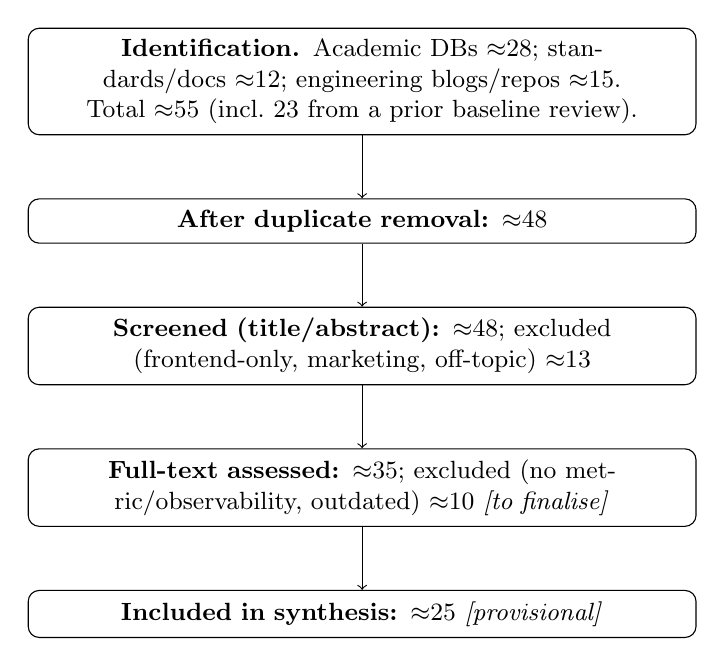
\begin{tikzpicture}[node distance=8mm, every node/.style={draw, rounded corners, align=center, font=\small, text width=8.2cm, inner sep=4pt}]
\node (id) {\textbf{Identification.} Academic DBs $\approx$28; standards/docs $\approx$12; engineering blogs/repos $\approx$15. Total $\approx$55 (incl.\ 23 from a prior baseline review).};
\node (dedup) [below=of id] {\textbf{After duplicate removal:} $\approx$48};
\node (screen) [below=of dedup] {\textbf{Screened (title/abstract):} $\approx$48; excluded (frontend-only, marketing, off-topic) $\approx$13};
\node (full) [below=of screen] {\textbf{Full-text assessed:} $\approx$35; excluded (no metric/observability, outdated) $\approx$10 \textit{[to finalise]}};
\node (inc) [below=of full] {\textbf{Included in synthesis:} $\approx$25 \textit{[provisional]}};
\draw[->] (id)--(dedup); \draw[->] (dedup)--(screen); \draw[->] (screen)--(full); \draw[->] (full)--(inc);
\end{tikzpicture}
\caption{PRISMA~2020 flow (provisional working counts).}
\label{fig:prisma}
\end{figure}

\subsection{Study Characteristics}
Table~\ref{tab:sources} lists representative included sources with their quality tier.

\begin{table}[H]
\centering\footnotesize
\caption{Representative included sources (tiered).}
\label{tab:sources}
\begin{tabularx}{\textwidth}{@{}l l c Y Y@{}}
\toprule
ID & Year & Tier & Focus & Metrics / contribution \\
\midrule
WWW'21 WebSocket adoption \cite{murley2021} & 2021 & T1 & WS in the wild (71k connections) & adoption, usage patterns \\
WS full-duplex eval \cite{ws2014} & 2014 & T1 & WS vs TCP & latency, network traffic \\
WS data transmission \cite{ws2019} & 2019 & T1 & WS RTC & throughput, latency \\
WS benchmark infra \cite{ws2016bench} & 2016 & T1 & server-side benchmark & black-box throughput \\
LLM serving eval \cite{arxivserving2025} & 2025 & T1 & LLM serving & TTFT, ITL, TPS, pitfalls \\
NVIDIA benchmarking \cite{nvidiabench2025} & 2025 & T2 & LLM serving & TTFT, ITL, TPS defs \\
Anyscale metrics \cite{anyscale2026} & 2026 & T2 & LLM serving & ITL formula \\
OTel GenAI semconv \cite{otelgenai2026} & 2026 & T2 & LLM observability & token-usage attributes \\
OneUptime SSE \cite{oneuptimesse2026} & 2026 & T3 & SSE tracing & connection+event span \\
OneUptime WS \cite{oneuptimews2026} & 2026 & T3 & WS tracing & cardinality problem \\
Alibaba LoongSuite \cite{alibabaws2026} & 2026 & T3 & WS observability & chunk metrics, agent \\
SSE vs WS for LLM \cite{buildmvpfast2026} & 2026 & T3 & transport choice & latency negligible \\
\bottomrule
\end{tabularx}
\end{table}

\subsection{Synthesis by Research Question}

\paragraph{RQ1 --- Metrics.} Two distinct layers emerge. \emph{Transport-level} (T1 academic): latency, throughput, bandwidth, CPU/memory, TCP connection count, and message frequency \cite{ws2014,ws2019,murley2021}. \emph{Token-level} (LLM serving): TTFT, ITL/TPOT, tokens/s, and end-to-end latency \cite{arxivserving2025,nvidiabench2025,anyscale2026}. The token-level set, not the REST set, is the relevant comparison basis for AI streaming.

\paragraph{RQ2 --- SSE vs WebSocket.} Evidence converges: for one-way server-to-client AI text streaming, SSE is sufficient and simpler (automatic reconnection, CDN compatibility, no sticky sessions), and is the choice of major LLM providers. The transport-level latency difference ($\approx$5--7\,ms) is negligible relative to per-token generation time ($\approx$10--12\,ms), so the model, not the transport, is the bottleneck \cite{buildmvpfast2026,procedure2026}. WebSocket is preferable when mid-stream bidirectional input is required (interruption, voice, collaboration) \cite{oneuptimews2026,getstream2026}.

\paragraph{RQ3 --- Tool support.} REST tracing is mature. LLM calls now have an emerging standard via the OpenTelemetry GenAI semantic conventions \cite{otelgenai2026}, but most attributes are experimental and do not yet cover the streaming lifecycle. SSE and WebSocket tracing still require deliberate, manual instrumentation \cite{oneuptimesse2026,oneuptimews2026,alibabaws2026}.

\paragraph{RQ4 --- Gaps.} Two recurring gaps: (i) after the handshake, frames/events carry no HTTP headers, breaking REST-style propagation; (ii) emitting one span per message or per token explodes span cardinality and overwhelms the collector \cite{oneuptimews2026}. Both motivate a \emph{two-tier} model: a connection-lifetime span plus a lightweight per-event/token record.

\paragraph{RQ5 --- Unified model.} The SSE pattern \cite{oneuptimesse2026} and the WebSocket pattern \cite{oneuptimews2026,alibabaws2026} independently converge on the same two-tier shape, yet no source offers a single, backend-independent, agent-free model that captures token-level metrics across both protocols. This is the gap this work targets.

%==============================================================
\section{Gap Analysis}
REST observability is mature because each request carries headers. SSE and WebSocket lack header-based per-message propagation and risk cardinality blow-up under naive per-message spans. The synthesis indicates a unified two-tier model --- one stream span anchoring per-event/token records --- applied identically to SSE and WebSocket, and exportable without a mandatory backend, would close the gap left by both agent-based tooling and protocol-specific tutorials.

%==============================================================
\section{Proposed Protocol-Aware Observability Framework}
We propose a five-layer framework (Table~\ref{tab:layers}) and a unified two-tier instrumentation model: each stream (SSE or WebSocket) is one connection-lifetime span, and each token/event is a lightweight \emph{span event} on that span, keeping span cardinality proportional to \emph{streams} rather than \emph{tokens}. Figure~\ref{fig:arch} shows the end-to-end architecture.

\begin{figure}[H]
\centering
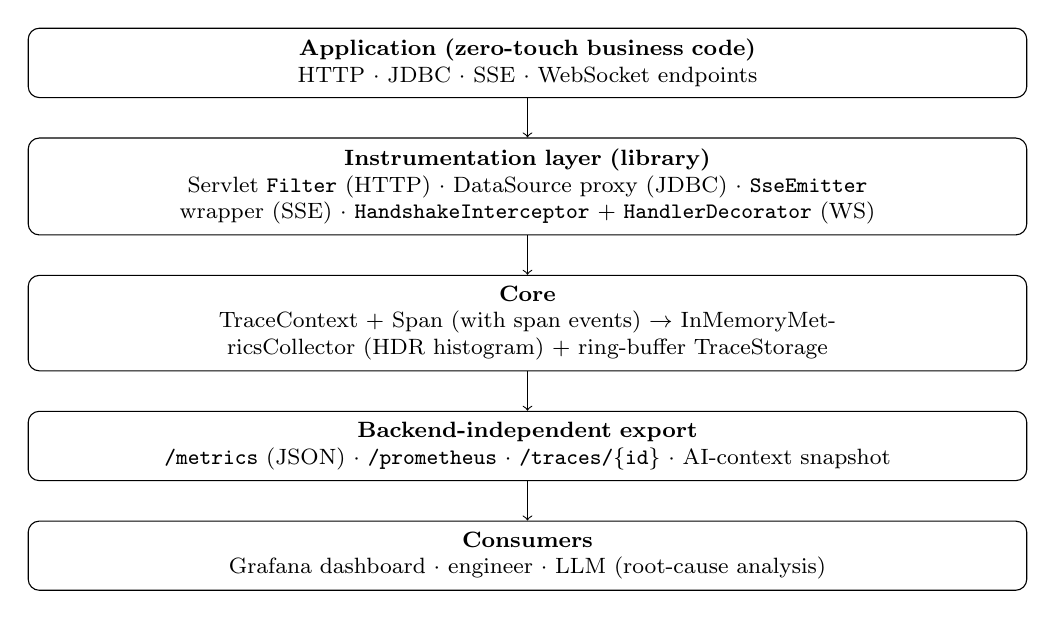
\begin{tikzpicture}[font=\footnotesize, node distance=5mm,
  box/.style={draw, rounded corners, align=center, inner sep=4pt, text width=12.4cm}]
\node[box] (app) {\textbf{Application (zero-touch business code)}\\ HTTP $\cdot$ JDBC $\cdot$ SSE $\cdot$ WebSocket endpoints};
\node[box, below=of app] (inst) {\textbf{Instrumentation layer (library)}\\ Servlet \texttt{Filter} (HTTP) $\cdot$ DataSource proxy (JDBC) $\cdot$ \texttt{SseEmitter} wrapper (SSE) $\cdot$ \texttt{HandshakeInterceptor} + \texttt{HandlerDecorator} (WS)};
\node[box, below=of inst] (core) {\textbf{Core}\\ TraceContext + Span (with span events) $\rightarrow$ InMemoryMetricsCollector (HDR histogram) + ring-buffer TraceStorage};
\node[box, below=of core] (out) {\textbf{Backend-independent export}\\ \texttt{/metrics} (JSON) $\cdot$ \texttt{/prometheus} $\cdot$ \texttt{/traces/\{id\}} $\cdot$ AI-context snapshot};
\node[box, below=of out] (cons) {\textbf{Consumers}\\ Grafana dashboard $\cdot$ engineer $\cdot$ LLM (root-cause analysis)};
\draw[->](app)--(inst);\draw[->](inst)--(core);\draw[->](core)--(out);\draw[->](out)--(cons);
\end{tikzpicture}
\caption{Architecture of the proposed protocol-aware observability library: zero-touch instrumentation feeds an in-memory core that exports without a mandatory backend.}
\label{fig:arch}
\end{figure}

\begin{table}[H]
\centering\small
\caption{Five-layer protocol-aware observability framework.}
\label{tab:layers}
\begin{tabularx}{\textwidth}{@{}l Y@{}}
\toprule
Layer & Signals \\
\midrule
L1 REST/API & request latency p50/p95/p99, throughput, error rate, payload size, status \\
L2 DB/downstream & JDBC latency, outbound latency, downstream error rate, cross-service span \\
L3 Streaming connection & active connections, connection duration, disconnect/timeout rate, completion rate \\
L4 Message/event & messages/events sent/received, chunk index, message size, events per stream \\
L5 AI streaming & TTFT, total stream duration, token throughput, user abort, provider latency \\
\bottomrule
\end{tabularx}
\end{table}

\subsection{Metric Catalogue}
We separate \emph{transport-level} metrics (used to compare SSE and WebSocket) from \emph{token/AI-level} metrics (used to characterise streaming quality, applied identically to both protocols). Table~\ref{tab:metrics} is the full catalogue; the core subset measured by the prototype is marked $\star$.

\begin{table}[H]
\centering\footnotesize
\caption{Metric catalogue. $\star$ = core subset for the prototype comparison.}
\label{tab:metrics}
\begin{tabularx}{\textwidth}{@{}l Y l l@{}}
\toprule
Metric & Formula & Unit & Source (tier) \\
\midrule
\multicolumn{4}{@{}l}{\textit{Transport-level}}\\
$\star$ Connection setup & $t_{\text{conn}} - t_{\text{req}}$ & ms & RFC 6455; IEEE WS (T1) \\
$\star$ Active connections & $\#\text{opened} - \#\text{closed}$ (gauge) & count & Alibaba WS (T3) \\
Stream duration & $t_{\text{close}} - t_{\text{open}}$ & ms & OneUptime (T3) \\
Throughput (bytes) & $B_{\text{total}} / W$ & bytes/s & WS thesis (T1) \\
$\star$ Latency pXX & $\mathrm{percentile}_{XX}(\{d_r\})$ & ms & HDR / Micrometer / Prometheus (T2) \\
Error/disconnect rate & $n_{\text{fail}} / n_{\text{total}} \times 100$ & \% & streaming refs (T2/T3) \\
\midrule
\multicolumn{4}{@{}l}{\textit{Token / AI-level}}\\
$\star$ TTFT & $t_1 - t_{\text{req}}$ & ms & NVIDIA, Anyscale (T2); arXiv (T1) \\
$\star$ Inter-token latency (ITL) & $\dfrac{t_N - t_1}{N-1}$ & ms/token & Anyscale, NVIDIA (T2) \\
$\star$ Output throughput & $\dfrac{N}{(t_N - t_{\text{req}})/1000}$ & tokens/s & NVIDIA, BentoML (T2) \\
End-to-end latency & $t_N - t_{\text{req}}$ & ms & arXiv (T1) \\
Inter-token jitter & $\mathrm{stddev}(\{t_{i+1}-t_i\})$ & ms & derived (smoothness) \\
Tokens per stream & $N$ & count & OTel GenAI semconv (T2) \\
\bottomrule
\end{tabularx}
\end{table}

\paragraph{Formal definitions.} Let $t_{\text{req}}$ be the request start time (client side), $t_{\text{conn}}$ the moment the connection is established, $t_1,\dots,t_N$ the client receive times of the $N$ streamed tokens, and $d_r$ the per-run latency observed over $r=1,\dots,R$ runs. The primary token-level metrics are:
\begin{align}
\text{TTFT} &= t_1 - t_{\text{req}}, &&[\text{ms}] \label{eq:ttft}\\
\text{ITL}  &= \frac{t_N - t_1}{N-1}, &&[\text{ms/token}] \label{eq:itl}\\
\text{Throughput} &= \frac{N}{(t_N - t_{\text{req}})/1000}, &&[\text{tokens/s}] \label{eq:tps}\\
\text{Jitter} &= \sqrt{\frac{1}{N-1}\sum_{i=1}^{N-1}\big((t_{i+1}-t_i) - \overline{\Delta t}\big)^2}, &&[\text{ms}] \label{eq:jitter}
\end{align}
where $\overline{\Delta t}$ is the mean inter-arrival gap. Equation~\eqref{eq:jitter} quantifies streaming smoothness: a high jitter at low ITL indicates stuttering output even when average speed is acceptable \cite{arxivserving2025}. Tail latency is reported as percentiles $\mathrm{p50/p95/p99}$ over $\{d_r\}$, computed with an HDR histogram rather than sort-on-query to bound memory and avoid $O(n\log n)$ per query \cite{micrometer2026,prometheushist2026}.

\paragraph{Measurement notes.} Four points must be fixed before any measurement is comparable.
\textbf{(1) Vantage point.} TTFT and ITL are measured \emph{client-side}, matching LLM-serving benchmark practice \cite{nvidiabench2025,anyscale2026}, because they reflect user-perceived responsiveness.
\textbf{(2) Controlled mock.} A deterministic generator emits a fixed $N$ with a fixed inter-token delay, so any measured difference between SSE and WebSocket is transport overhead rather than model variance.
\textbf{(3) ITL definition.} Tools differ on whether the first token is included; we exclude it (Eq.~\eqref{eq:itl} divides by $N-1$), since TTFT already captures the first-token cost \cite{arxivserving2025,anyscale2026}.
\textbf{(4) SSE latency skew.} An SSE stream is one long-lived HTTP response, so measuring it as a REST ``request latency'' yields a duration equal to the stream lifetime, distorting p95/p99; latency must therefore be measured per token/event, not per request --- a protocol-aware requirement rather than an implementation detail.

\subsection{Prototype Scope}
A minimal Java/Spring~Boot prototype instruments REST (Filter/Interceptor), JDBC (DataSource proxy), SSE (an \texttt{SseEmitter} wrapper), and WebSocket (\texttt{HandshakeInterceptor} + \texttt{WebSocketHandlerDecorator}), recording each token as a span event under a single stream span. A deterministic mock token generator (fixed token count and inter-token delay) isolates transport overhead from model latency, enabling a fair SSE-vs-WebSocket comparison on identical input. Metrics are exposed as JSON; no external collector or real LLM provider is required. SSE notably lacks a global instrumentation hook (unlike the Servlet filter or WebSocket decorator), so it must wrap the emitter --- itself a finding for RQ3/RQ4.

%==============================================================
\section{Discussion}
Protocol choice should follow workload, not trend: SSE is adequate and simpler for one-way token streaming, while WebSocket is justified by bidirectional interaction. The more consequential issue is observability: streaming systems require protocol-aware, message/token-level instrumentation that header-based REST tracing cannot provide. A backend-independent, agent-free library is attractive for legacy or self-hosted RAG deployments where bytecode agents and full OpenTelemetry backends are undesirable, complementing agent-based solutions such as LoongSuite \cite{alibabaws2026} rather than competing on depth.

\subsection{Comparison with Closest Work}
Table~\ref{tab:compare} contrasts this work with the nearest existing approaches across the dimensions a practitioner cares about. No existing approach combines an agent-free, backend-independent design with a single token-level model spanning both SSE and WebSocket.

\begin{table}[H]
\centering\footnotesize
\caption{Comparison with the closest existing approaches.}
\label{tab:compare}
\begin{tabular}{@{}lcccc@{}}
\toprule
Dimension & OTel + GenAI \cite{oteldocs,otelgenai2026} & LoongSuite \cite{alibabaws2026} & OneUptime \cite{oneuptimesse2026,oneuptimews2026} & This work \\
\midrule
Agent-free            & No      & No      & Yes (manual SDK) & Yes \\
Backend-independent   & No      & No      & No               & Yes \\
SSE support           & Partial & No      & Yes              & Yes \\
WebSocket support     & Partial & Yes     & Yes              & Yes \\
Token-level metrics   & Partial & Partial & Partial          & Yes \\
Unified SSE+WS model  & No      & No      & No               & Yes \\
LLM-readable export   & No      & No      & No               & Yes \\
\bottomrule
\end{tabular}
\end{table}

\subsection{Scalability Considerations}
The two-tier model bounds span cardinality by the number of \emph{concurrent streams}, not by message or token volume: per-stream memory is one span plus lightweight span events, and per-endpoint metrics use fixed-size HDR histograms, so metric memory is independent of request count. Trace storage is a fixed-capacity ring buffer that evicts the oldest entries. The library is therefore expected to scale comfortably to moderate concurrency; at very high concurrency (e.g.\ $10^4$--$10^5$ simultaneous streams), the per-session context map and active-connection bookkeeping dominate memory and trace sampling becomes necessary, while cross-process aggregation would rely on the optional Prometheus export rather than the in-memory store. These are analytical expectations; quantitative load testing is left to future work.

%==============================================================
\section{Limitations (Threats to Validity)}
The review is preliminary: PRISMA counts are provisional and no benchmark has yet been run. Much of the SSE-vs-WebSocket-for-LLM evidence is T3 (engineering blogs) rather than peer-reviewed --- a finding in itself about the immaturity of academic coverage --- and is treated as current practice, not proof. TTFT/ITL definitions vary across tools, so any future measurement must state the exact formula used. The proposed framework still requires validation through implementation.

%==============================================================
\section{Conclusion and Future Work}
This preliminary, PRISMA-guided review finds that token-level streaming metrics are well defined, that SSE and WebSocket differ little for one-way token streaming, and that no unified, backend-independent, agent-free model captures token-level observability across both protocols. We propose a five-layer framework and a two-tier instrumentation model, with a Java/Spring~Boot prototype scope.

Near-term future work completes the search and screening (finalising the PRISMA counts), implements the SSE adapter and the deterministic mock workload, and reports measured TTFT, ITL, throughput, jitter, and connection metrics comparing SSE and WebSocket under controlled conditions, including a load/scalability test at increasing concurrency. Longer-term extensions include: additional streaming transports (gRPC streaming, HTTP/3 over QUIC, Kafka-based event streaming); tracing for emerging AI-agent protocols such as the Model Context Protocol (MCP) and multi-agent pipelines; an OTLP bridge for interoperability with existing backends; adaptive sampling; and a production deployment study.

\begin{thebibliography}{99}
\bibitem{prisma2020} M.~J. Page et al., ``The PRISMA 2020 statement,'' \emph{BMJ}, 2021. \url{https://www.prisma-statement.org/}
\bibitem{murley2021} P.~Murley et al., ``WebSocket Adoption and the Landscape of the Real-Time Web,'' \emph{Proc. Web Conf. (WWW)}, 2021. \url{https://faculty.cc.gatech.edu/~mbailey/publications/www21_websocket.pdf}
\bibitem{ws2014} ``Performance evaluation of WebSocket protocol for full-duplex web streams,'' \emph{IEEE MIPRO}, 2014. \url{https://ieeexplore.ieee.org/document/6859715}
\bibitem{ws2019} ``Performance Analysis of Data Transmission on WebSocket for Real-time Communication,'' \emph{IEEE}, 2019. \url{https://ieeexplore.ieee.org/document/8898135/}
\bibitem{ws2016bench} ``Introduction to a WebSocket benchmarking infrastructure,'' \emph{IEEE}, 2016. \url{https://ieeexplore.ieee.org/document/7513661/}
\bibitem{arxivserving2025} ``On Evaluating Performance of LLM Inference Serving Systems,'' arXiv:2507.09019, 2025. \url{https://arxiv.org/pdf/2507.09019}
\bibitem{nvidiabench2025} NVIDIA, ``LLM Inference Benchmarking: Fundamental Concepts,'' 2025. \url{https://developer.nvidia.com/blog/llm-benchmarking-fundamental-concepts/}
\bibitem{anyscale2026} Anyscale, ``Understand LLM latency and throughput metrics,'' 2026. \url{https://docs.anyscale.com/llm/serving/benchmarking/metrics}
\bibitem{otelgenai2026} OpenTelemetry, ``Semantic conventions for generative AI spans,'' 2026. \url{https://opentelemetry.io/docs/specs/semconv/gen-ai/gen-ai-spans/}
\bibitem{oneuptimesse2026} OneUptime, ``Monitor SSE Stream Lifecycle and Delivery Latency with OpenTelemetry,'' 2026. \url{https://oneuptime.com/blog/post/2026-02-06-sse-stream-lifecycle-opentelemetry/view}
\bibitem{oneuptimews2026} OneUptime, ``Trace WebSocket Connections and Real-Time Events with OpenTelemetry,'' 2026. \url{https://oneuptime.com/blog/post/2026-02-06-trace-websocket-connections-realtime-events-opentelemetry/view}
\bibitem{alibabaws2026} Alibaba Cloud, ``Master WebSocket End-to-end Observability in One Article,'' 2026. \url{https://www.alibabacloud.com/blog/master-websocket-end-to-end-observability-in-one-article_602915}
\bibitem{splunkws2023} Splunk, ``Instrumenting Java WebSocket Messaging,'' 2023. \url{https://community.splunk.com/t5/Community-Blog/Instrumenting-Java-Websocket-Messaging/ba-p/629425}
\bibitem{buildmvpfast2026} ``SSE vs WebSockets for Streaming LLM Responses,'' 2026. \url{https://www.buildmvpfast.com/blog/streaming-llm-responses-sse-vs-websockets-2026}
\bibitem{procedure2026} Procedure, ``Why Server-Sent Events Still Win for LLM Streaming,'' 2026. \url{https://procedure.tech/blogs/the-streaming-backbone-of-llms-why-server-sent-events-(sse)-still-wins-in-2025}
\bibitem{getstream2026} GetStream, ``WebSocket vs Server-Sent Events,'' 2026. \url{https://getstream.io/blog/websocket-sse/}
\bibitem{rfc6455} I.~Fette and A.~Melnikov, ``The WebSocket Protocol,'' RFC 6455, IETF, 2011. \url{https://datatracker.ietf.org/doc/html/rfc6455}
\bibitem{whatwgsse} WHATWG, ``Server-sent events,'' HTML Living Standard. \url{https://html.spec.whatwg.org/multipage/server-sent-events.html}
\bibitem{w3ctrace} W3C, ``Trace Context,'' W3C Recommendation, 2021. \url{https://www.w3.org/TR/trace-context/}
\bibitem{oteldocs} OpenTelemetry Documentation. \url{https://opentelemetry.io/docs/}
\bibitem{dapper2010} B.~H. Sigelman et al., ``Dapper, a Large-Scale Distributed Systems Tracing Infrastructure,'' Google, 2010. \url{https://research.google.com/archive/papers/dapper-2010-1.pdf}
\bibitem{micrometer2026} Micrometer, ``Histograms and percentiles.'' \url{https://docs.micrometer.io/micrometer/reference/concepts/histogram-quantiles.html}
\bibitem{prometheushist2026} Prometheus, ``Histograms and summaries.'' \url{https://prometheus.io/docs/practices/histograms/}
\end{thebibliography}

\end{document}
